\chapter{High-Level Design}

The Intelligent Clinical Document Processing System (ICDPS) consists of multiple components that work together to process clinical documents, extract relevant information, generate summaries, and map identified entities to SNOMED CT concepts. To support these operations, the system is organized as a modular processing pipeline in which each component performs a specific task and passes its output to the next stage.

This chapter describes the overall architecture of the proposed system, the design principles considered during development, and the high-level interactions between major modules. The architecture provides a framework for understanding how clinical documents move through the system from ingestion to final review and coding.

\section{Design Considerations}

Several design considerations influenced the architecture of the ICDPS. Since clinical documents may vary in format, content, and quality, the system was designed to support flexible document processing while maintaining reliability and ease of maintenance. Additional considerations included scalability, security, modularity, and support for future extensions.

These factors guided the selection of technologies, deployment strategies, and interactions between individual system components.

\subsection{General Considerations}

The architectural design of the ICDPS was guided by the following engineering principles:

\begin{itemize}

\item \textbf{Modularity:} The system is decomposed into independently deployable modules --- Document Ingestion, Text Extraction, NER Engine, Summarization Engine, SNOMED CT Mapper, and Review Interface --- each with well-defined input and output contracts. This modular structure supports component-level testing, independent updates, and replacement of individual technologies without affecting the entire system.

\item \textbf{Scalability:} The processing pipeline supports horizontal scaling through containerized deployment. Additional processing instances can be introduced when document throughput requirements increase.

\item \textbf{Reliability:} Error-handling mechanisms are incorporated at each stage of the pipeline. Documents that fail processing are redirected to an error queue for review, and processing events are recorded for auditing and troubleshooting.

\item \textbf{Maintainability:} Modules are documented using API specifications and maintained within a version-controlled repository. Configuration files and model weights are managed separately from application code to simplify updates and maintenance.

\item \textbf{Security:} Role-based access control is enforced for system interfaces and API endpoints. Clinical documents and extracted information are processed within the deployment environment, with access restricted to authorized users.

\item \textbf{Explainability:} SNOMED CT code suggestions are accompanied by confidence scores, and extracted entities are linked to their corresponding text spans to support user review and verification.

\end{itemize}

\subsection{Development Methodology}

Development followed an iterative Software Development Life Cycle (SDLC) consisting of requirements analysis, system design, implementation, testing, and deployment preparation. This approach allowed individual components to be developed and evaluated incrementally, with modifications introduced based on intermediate testing and performance results.

Agile development practices, including periodic sprint reviews, version control, and continuous integration through GitHub Actions, were used to monitor progress and manage development activities throughout the project.

\section{Architecture Strategies}

Architecture strategies describe the structural and technological approaches used in the development of the proposed system. These decisions influence how components communicate, how data moves through the processing pipeline, and how the system can be extended or deployed in different environments.

The selected architecture combines document processing, NLP, semantic retrieval, and terminology mapping within a modular framework. This design allows individual components to be updated independently while maintaining compatibility with the overall processing workflow.

\subsection{Technology and Framework Selection}
Python 3.10 was chosen as the primary implementation language because of its extensive support for machine learning, natural language processing, and data processing libraries. It also provides compatibility with the frameworks and tools used throughout the project. The Hugging Face Transformers library was selected as the primary NLP framework because it offers well-documented implementations of BioBERT and other transformer-based models, along with standardized interfaces for training and inference.

PyMuPDF was selected for PDF text extraction due to its superior text extraction fidelity on complex clinical PDF layouts compared to alternatives such as pdfplumber and PDFMiner. Tesseract 5.0 was selected for OCR because it supports LSTM-based recognition with NHS-relevant font coverage and is available under a free and open-source licence.

FAISS was selected for SNOMED CT vector search because it provides both exact and approximate nearest-neighbour search with GPU acceleration support, enabling sub-second retrieval from the 1.5 million concept description index. Flask was selected for the web interface due to its lightweight architecture suitable for the single-institution deployment context.

\subsection{Scalability and Future Enhancements}
The containerized architecture supports future deployment on cloud infrastructure (NHS-approved cloud providers). Additional NLP models supporting ICD-10 or LOINC coding could be integrated as independent modules without modifying the core pipeline. The SNOMED CT index can be updated to reflect new SNOMED CT releases by rerunning the index construction script with the new release files.

Future enhancements identified include:
\begin{enumerate}[(i)]
    \item real-time API integration with NHS EHR systems;
    \item support for handwritten clinical note processing using dedicated handwriting recognition models;
    \item multilingual support for Welsh and other NHS-relevant languages; and
    \item active learning integration to continuously improve extraction performance using clinician feedback.
\end{enumerate}

\section{Overall System Architecture}

The Intelligent Clinical Document Processing System (ICDPS) processes clinical documents through a sequence of interconnected stages that transform raw documents into structured clinical information and SNOMED CT coding suggestions. The system is designed to handle documents originating from different sources, including scanned reports, referral letters, discharge summaries, and other healthcare records that may vary in format and quality.

To support this workflow, the architecture is organized into multiple processing layers. Each layer performs a specific task and passes its output to the next stage of the pipeline. This modular structure simplifies development and testing while allowing individual components to be updated or replaced without affecting the overall workflow.

\subsection{High-Level Architecture Diagram}

Figure~\ref{fig:hla_diagram} illustrates the overall processing workflow of the ICDPS. The workflow begins with document ingestion and concludes with the presentation of extracted information, summaries, and coding suggestions through the NHS Portal interface. The architecture is organized into six primary processing layers, each responsible for a distinct stage of document analysis.

\textbf{Layer 1 --- Document Ingestion and Rendering} receives uploaded clinical documents through the NHS Portal interface. Documents are processed by the \texttt{document\_handler} module and routed to PyMuPDF for page-level rendering and conversion into PNG images for downstream processing.
\textbf{Layer 2 --- Image Preprocessing} uses OpenCV to improve image quality before OCR processing. Operations such as adaptive thresholding, noise reduction, and deskewing are applied to improve text visibility and document consistency.

\textbf{Layer 3 --- OCR Extraction and Confidence Routing} uses AWS Textract to extract document text and confidence values. Documents with confidence scores above the predefined threshold continue through the standard processing path, while lower-confidence outputs are forwarded to a LayoutLMv3 refinement stage.

\textbf{Layer 4 --- Entity Extraction and Clinical Coding} identifies clinically relevant entities and maps extracted concepts to SNOMED CT terminology using the clinical coding pipeline.

\textbf{Layer 5 --- PHI Detection, Structured Field Extraction, and Summarisation} detects protected health information (PHI), extracts structured fields, and generates summaries tailored to different user roles.

\textbf{Layer 6 --- Confidence Aggregation and Output Rendering} combines confidence measures from multiple processing stages to calculate a Unified Confidence Score (UCS) and presents the final results through the NHS Portal interface.

\begin{figure}[htbp]
\centering
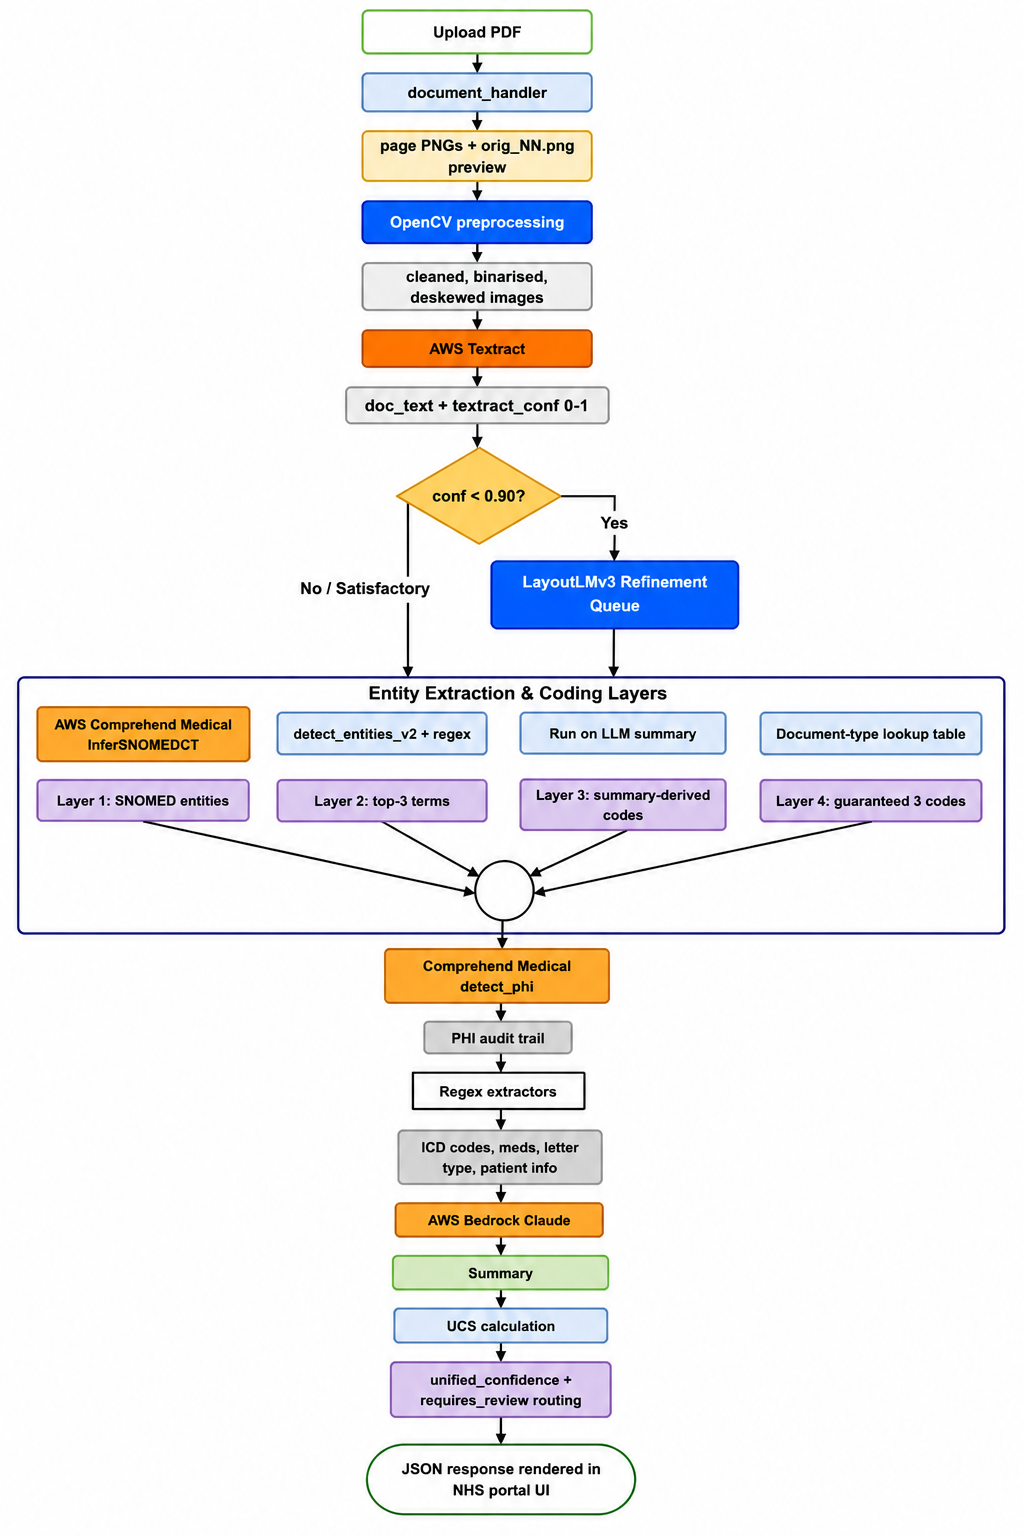
\includegraphics[width=\textwidth]{Figures/hla_diagram.png}
\caption{High-Level Architecture Diagram of the ICDPS six-layer processing pipeline.}
\label{fig:hla_diagram}
\end{figure}

\subsection{Module Description}

The ICDPS consists of a set of modules that collectively implement the document processing workflow. Each module is responsible for a specific stage of processing and exchanges information with other components through predefined interfaces. This separation allows individual modules to be modified, optimized, or extended independently as the system evolves.

Table~\ref{tab:module_descriptions} summarizes the major modules in the architecture, along with their inputs, processing responsibilities, and generated outputs.

\begin{longtable}{|>{\raggedright\arraybackslash}p{3.3cm}|
                  >{\raggedright\arraybackslash}p{2.7cm}|
                  >{\raggedright\arraybackslash}p{3.9cm}|
                  >{\raggedright\arraybackslash}p{3.9cm}|}
\caption{ICDPS Module Descriptions}
\label{tab:module_descriptions} \\
\hline
\textbf{Module} & \textbf{Input} & \textbf{Processing} & \textbf{Output} \\
\hline
\endfirsthead
\hline
\textbf{Module} & \textbf{Input} & \textbf{Processing} & \textbf{Output} \\
\hline
\endhead
\hline
\endfoot
\texttt{document\_handler} & PDF / JPEG / PNG / TIFF & PyMuPDF rendering; file type routing & PNG page images; \texttt{orig\_NN.png} previews \\
\hline
OpenCV Preprocessor & Raw page PNGs & Adaptive threshold; MORPH\_CLOSE; deskew & Cleaned, binarised, aligned PNGs \\
\hline
AWS Textract OCR & Preprocessed PNGs & AnalyzeDocument API; block parsing & \texttt{doc\_text}; \texttt{textract\_conf} (0--1) \\
\hline
Confidence Router & \texttt{textract\_conf} & Threshold comparison vs.\ 0.90 & Route to LayoutLMv3 or continue \\
\hline
LayoutLMv3 Refiner & Low-conf page images & Multi-modal transformer inference & Corrected text blocks \\
\hline
SNOMED Mapper (4-layer) & \texttt{doc\_text}; entities; summary & InferSNOMEDCT; regex; lookup table & SNOMED codes with confidence \\
\hline
PHI Detector & \texttt{doc\_text} & Comprehend Medical DetectPHI & \texttt{phi\_entities} list; audit trail \\
\hline
Regex Extractor & \texttt{doc\_text} & Pattern matching for ICD-10, meds & \texttt{icd\_codes}; medications; patient info \\
\hline
Bedrock Claude LLM & \texttt{doc\_text} + SNOMED entities & Role-specific prompts; prose generation & 3 role-specific summaries \\
\hline
UCS Calculator & \texttt{textract\_conf}; \texttt{snomed\_conf}; \texttt{llm\_conf} & Weighted formula by document type & \texttt{unified\_confidence}; review routing \\
\hline
NHS Portal UI & JSON result dict & JavaScript / React rendering & Interactive clinical review interface \\
\hline
\end{longtable}

\subsection{High-Level AI Workflow}

The AI workflow within the ICDPS processes extracted document content through multiple analysis paths rather than a single sequential pipeline. After OCR extraction, the document content is routed to two independent processing tracks together with a confidence evaluation mechanism.

\begin{itemize}

\item \textbf{Track A} performs clinical entity extraction and terminology mapping. Extracted medical concepts are processed through the SNOMED CT safety-net architecture to identify appropriate standardized healthcare codes.

\item \textbf{Track B} performs clinical language understanding and document summarization. AWS Bedrock Claude Sonnet is used to generate contextual summaries tailored to different healthcare users and review scenarios.

\item \textbf{Confidence Scoring Layer} combines confidence values generated during OCR extraction, SNOMED CT mapping, and language model processing. These values are aggregated into a Unified Confidence Score (UCS), which is used to determine whether the generated output can proceed automatically or requires additional human review.

\end{itemize}

The separation of entity extraction and language understanding into independent processing tracks allows the system to continue producing useful outputs even when one component performs less effectively on a particular document.

\section{Data and Learning Workflow}

The ICDPS workflow describes how information moves through the system during both training and inference. Clinical documents are progressively transformed from raw uploaded files into structured entities, summaries, and SNOMED CT coding suggestions through a sequence of processing stages.

The workflow includes document ingestion, OCR processing, information extraction, terminology mapping, confidence evaluation, and output generation. Each stage produces intermediate results that are passed to downstream components, allowing individual modules to be evaluated, updated, and maintained independently.

The following sections describe the flow of data through the system and the learning processes used to train and evaluate the machine learning components.

\subsection{End-to-End Workflow Diagram}
The end-to-end workflow provides a comprehensive representation of the sequence of operations performed by ICDPS from document submission to final output generation. The complete process is divided into five major stages:

\begin{enumerate}
    \item Document Upload and Ingestion
    \item Image Preprocessing
    \item OCR Extraction and Confidence Routing
    \item Parallel Processing for Entity Extraction, PHI Detection, and Summarisation
    \item Confidence Aggregation and Output Rendering
\end{enumerate}

Each stage produces outputs that are passed to downstream components, forming the overall document processing workflow. The process begins when a clinical document is uploaded through the NHS Portal interface. Document pages are rendered and enhanced before OCR extraction converts visual content into machine-readable text. Confidence-based routing is then used to determine whether additional processing through the LayoutLMv3 refinement module is required. After text extraction, multiple downstream tasks execute in parallel to reduce processing time and improve overall throughput.

\subsection{Training Workflow Overview}

Most components within the ICDPS rely on pre-trained models and managed services for OCR, language understanding, and terminology processing. As a result, large-scale model training is not required for every stage of the pipeline. However, the LayoutLMv3 refinement module was adapted for clinical document processing through task-specific fine-tuning.

The training workflow begins with the collection and preparation of NHS-style clinical documents. Documents are converted into annotated page images and associated with bounding-box information representing relevant text regions. The dataset is divided into training, validation, and testing subsets using a 70:15:15 split.

A pre-trained LayoutLMv3-base model is then fine-tuned using the AdamW optimizer together with cosine annealing learning-rate scheduling. Validation performance is evaluated throughout training, and early stopping is used to reduce overfitting. The checkpoint achieving the best validation performance is selected for deployment within the refinement stage of the production pipeline.

\subsection{Inference Workflow Overview}

The inference workflow describes how the deployed system processes newly submitted clinical documents. Unlike the training workflow, no model parameters are updated during this stage.

When a document is uploaded, it undergoes rendering and image preprocessing before being submitted to AWS Textract for OCR extraction. Documents with OCR confidence scores above the predefined threshold of 0.90 continue through the standard processing path. Documents falling below this threshold are routed to the LayoutLMv3 refinement module for additional processing.

Following text extraction, the SNOMED CT mapping cascade identifies medical concepts and generates standardized terminology suggestions. PHI detection, structured field extraction, and document summarization execute in parallel to improve processing efficiency. The resulting outputs are then combined with confidence measures from multiple stages to calculate the Unified Confidence Score (UCS). Based on this score, the system determines whether the generated results can proceed directly to output generation or should be flagged for clinician review.

\section{System Interaction and Deployment Overview}

This section describes how users interact with the ICDPS platform and how the system components operate within the deployment environment. In addition to document processing functionality, the platform must support secure data handling, responsive user interaction, and reliable execution of the processing pipeline. The deployment architecture combines containerized services and cloud infrastructure to support document processing, model inference, and workflow management.

\subsection{User Interaction Flow}

The NHS Portal UI serves as the primary interface through which healthcare users interact with the system. The interface supports document submission, review of generated outputs, and export of processed results.

When a document is uploaded, a multipart POST request initiates the backend processing workflow. Processing status is communicated through a progress indicator while the document moves through the pipeline. After processing is complete, results are presented through four tabbed views: Details, Coding, Follow-up, and GP Actions.

A colour-coded Unified Confidence Score badge provides a visual indication of output confidence. Users can review generated summaries, inspect extracted entities, modify SNOMED CT coding suggestions where necessary, and export the resulting structured records.

\subsection{Model-Service Interaction}

Communication between processing components is handled through secure service interfaces. The ICDPS backend interacts with AWS services through \texttt{boto3} clients using encrypted TLS connections and region-specific endpoints. Deploying related services within the same AWS region helps reduce communication latency and simplifies operational management.

Protected Health Information (PHI) is excluded from logging operations before audit records are stored. The LayoutLMv3 refinement component is deployed as a locally hosted containerized service, enabling independent inference and asynchronous processing of low-confidence documents.

\subsection{Deployment Overview}

The ICDPS deployment architecture uses a cloud-native approach built around containerized services and managed AWS infrastructure. The Flask backend and LayoutLMv3 inference service are packaged using Docker containers and deployed through Amazon ECS with Fargate support.

The NHS Portal frontend is distributed through CloudFront to improve availability and response times. Amazon SQS provides asynchronous communication between processing stages, while AWS Step Functions coordinate workflow execution and error-handling procedures. Audit records, extracted information, and processing metadata are stored in Amazon DynamoDB.

This deployment model separates processing responsibilities across multiple services while supporting scalability, fault tolerance, and operational flexibility.

\section*{Summary}

This chapter described the high-level architecture of the Intelligent Clinical Document Processing System (ICDPS), including the major processing layers, module interactions, AI workflow, deployment environment, and user interaction mechanisms. The design principles adopted during development and the technologies used to implement the architecture were also discussed.

The architecture provides a framework for understanding how clinical documents move through the system from ingestion to final output generation. The next chapter presents the detailed design of individual modules, including data organization, preprocessing workflows, model configurations, and implementation-level design decisions.
